\documentclass[11pt]{article}

\usepackage[letterpaper,margin=0.5in]{geometry}
\usepackage{amsmath}
\usepackage{amssymb}
\usepackage{dsfont}
\usepackage{bbm}
\usepackage{stmaryrd}
\usepackage{graphicx}
\usepackage{pbox}
\usepackage{hyperref}
\usepackage{changepage}


\newcommand{\braces}[1]{\left\{#1\right\}}
\newcommand{\abs}[1]{\left|#1\right|}
\renewcommand{\vec}[1]{\mathbf{#1}}
\newcommand{\mean}[1]{\langle #1 \rangle}
\newcommand{\norm}[1]{\left|\left|{#1}\right|\right|}

\newcommand{\beq}{\begin{equation}}
\newcommand{\eeq}{\end{equation}}
\newcommand{\beqa}{\begin{eqnarray}}
\newcommand{\eeqa}{\end{eqnarray}}
\newcommand{\beqaN}{\begin{eqnarray*}}
\newcommand{\eeqaN}{\end{eqnarray*}}

\newcommand{\micron}{\mu\textrm{m}}
\newcommand{\specialcell}[2][c]{%
  \begin{tabular}[#1]{@{}c@{}}#2\end{tabular}}

\newcommand{\boldrho}{\rho\hspace{-5.1pt}\rho}
% \newcommand{\grvec}[1]{#1\hspace{-6pt}#1\hspace{-6pt}#1\hspace{1pt}}
\newcommand{\grvec}[1]{\boldsymbol{#1}}
\newcommand{\one}{\mathds{1}}

\newcommand{\hp}{\circ}%{\odot}%{\circ}
\newcommand{\hd}{\hspace{-1.6mm}\fatslash}%{\oslash}'

\setlength{\parskip}{1em}
\setlength{\parindent}{0in}

\begin{document}

\author{Ahmadreza Ghaffarizadeh, Samuel H. Friedman, Paul Macklin${}^*$}
\title{BioFVM: an efficient, parallelized diffusive transport solver for 3-D biological simulations
\break\break
\textbf{\huge{Tutorial}}
}
\date{}
\date{Revision: July 19, 2017}	

\maketitle
This tutorial will teach you how to download, install and run a series of biological problems in BioFVM.
Please note that this tutorial will be periodically updated.
Users should check \href{http://BioFVM.MathCancer.org}{BioFVM.MathCancer.org}  for the latest version. BioFVM manuscript 
is currently under review by \textit{Bioinformatics} journal; please see the the citation information below.


% [problem statement] In this paper, we introduce BioFVM, an open source C++
% solver for systems of 3-D reaction-diffusion equations, solved using the finite volume
% method (FVM). We include functions for off-lattice, cell-centered substrate sources and sinks,
% as are commonly required in multicellular simulations.
% The code has been optimized for use on modern multithreaded processors, and
% parallelized with OpenMP. Its computational cost scales linearly with the number of substrates
% simulated and the spatial domain size and resolution.
% We provide several examples demonstrating
% BioFVM's scalability to simulations with 1-10 substrates on 1-10 million computational voxels
% on high-end desktop computers, with second-order spatial accuracy and first-order time accuracy.
% This code is well-documented and freely available under the GPL 2.0 at http://MathCancer.org.
% }

% Target journal: Application note in Bioinformatics

%\begin{abstract}
%\noindent
%These are the supplementary materials for: \\
%
%\begin{center}
%\parbox[t]{15cm}{A. Ghaffarizadeh, S.H. Friedman, and P. Macklin, \textbf{BioFVM: an efficient parallelized diffusive transport solver
%for 3-D biological simulations,} \emph{Bioinformatics.} (2015, in review)\\}
%\end{center}
%
%\noindent
%Any corrections will be posted online at \href{http://BioFVM.MathCancer.org}{BioFVM.MathCancer.org}\\
%
%\noindent
%\textbf{Motivation:} Computational models of multicellular systems require solving systems
%of PDEs for release, uptake, decay, and diffusion of multiple substrates in 3D, particularly when
%incorporating the impact of drugs, growth substrates, and signaling factors on cell receptors and subcellular systems biology. \\
%\textbf{Results:} We introduce BioFVM, a diffusive transport solver tailored to biological problems.
%BioFVM can simulate release and uptake of many substrates by cell and bulk sources, diffusion,
%and decay in large 3D domains.  It has been % optimized and
%parallelized with OpenMP, allowing efficient simulations on desktop workstations or single supercomputer nodes.
%The code is stable even for large time steps, with linear computational cost scalings.
%Solutions are first-order accurate in time and second-order accurate in space.
%The code can be run by itself or as part of a
%larger simulator.\\
%\textbf{Availability:} BioFVM is written in C++ with parallelization in OpenMP.
%It is maintained and available for download at \href{http://BioFVM.MathCancer.org}{http://BioFVM.MathCancer.org} and \href{http://BioFVM.sf.net}{http://BioFVM.sf.net} under the
%Apache License (v2.0). \\
%\textbf{Contact:} \href{paul.macklin@usc.edu}{paul.macklin@usc.edu}\\
%\textbf{Supplementary information:} The full algorithm and convergence/performance testing are provided in supplementary materials and at \href{http://BioFVM.MathCancer.org}{BioFVM.MathCancer.org}. A tutorial is included in each BioFVM download.
%\end{abstract}



\section{Citing BioFVM}
If you use BioFVM in your project, please cite BioFVM and the version  number, such as below:\\



\begin{adjustwidth}{2.5em}{0pt}
We solved the diffusion equations using BioFVM (Version 1.1.5) [1]. 

[1] A. Ghaffarizadeh, S.H. Friedman, and P. Macklin, BioFVM: an efficient parallelized diffusive transport solver for 3-D biological simulations, \emph{Bioinformatics} 32(8):1256-8, 2016. 
DOI: \href{http://dx.doi.org/10.1093/bioinformatics/btv730}{10.1093/bioinformatics/btv730}.
\end{adjustwidth}


\section{Preparing to use BioFVM}
\subsection{Downloading BioFVM}
BioFVM is available at \href{http://BioFVM.MathCancer.org}{BioFVM.MathCancer.org} and at \href{http://BioFVM.sf.net}{BioFVM.sf.net}.
Because we aim for cross-platform compatibility and simplicity, we designed BioFVM
to minimize external dependencies.  As of Version 1.0, the only external library is pugixml (included in the download).

\subsection{Supported platforms}
BioFVM should successfully compile and run on any C++11 or later compiler that supports OpenMP.
We recommend using a 64-bit compiler for best results. We target g++ (Version 4.8.4 or later)
on Linux and OSX, and MinGW-W64(gcc version 4.9.0 or later) on Windows for this version (testing and support are planned
for the Intel C++ compiler in the future versions).

\subsection{Including BioFVM in a project}
\label{including_biofvm}
BioFVM does not require any form of installation for use in a project. Instead, extract all
its cpp and h files in your project directory. All BioFVM source files begin with the prefix
``\verb:BioFVM_:''. If your project uses makefiles, you'll want to include
the following lines:

\begin{verbatim}
CC     := g++       # replace with your compiler
ARCH := core2 # a reasonably safe default for most CPUs since 2007
# ARCH := corei7
# ARCH := corei7-avx # earlier i7
# ARCH := core-avx-i # i7 ivy bridge or newer
# ARCH := core-avx2 # i7 with Haswell or newer
# ARCH := nehalem
# ARCH := westmere
# ARCH := sandybridge
# ARCH := ivybridge
# ARCH := haswell
# ARCH := broadwell
# ARCH := bonnell
# ARCH := silvermont
# ARCH := nocona #64-bit pentium 4 or later

CFLAGS := -march=$(ARCH) -O3 -s -fomit-frame-pointer -mfpmath=both -fopenmp -m64 -std=c++11
# replace CFLAGS as you see necessary, but make sure to use -std=c++11 -fopenmp

BioFVM_OBJECTS := BioFVM_vector.o BioFVM_matlab.o BioFVM_utilities.o BioFVM_mesh.o \
BioFVM_microenvironment.o BioFVM_solvers.o BioFVM_basic_agent.o \
BioFVM_agent_container.o BioFVM_MultiCellDS.o 

COMPILE_COMMAND := $(CC) $(CFLAGS)

BioFVM_vector.o: BioFVM_vector.cpp
	$(COMPILE_COMMAND) -c BioFVM_vector.cpp

BioFVM_agent_container.o: BioFVM_agent_container.cpp
	$(COMPILE_COMMAND) -c BioFVM_agent_container.cpp
	
BioFVM_mesh.o: BioFVM_mesh.cpp
	$(COMPILE_COMMAND) -c BioFVM_mesh.cpp

BioFVM_microenvironment.o: BioFVM_microenvironment.cpp
	$(COMPILE_COMMAND) -c BioFVM_microenvironment.cpp

BioFVM_solvers.o: BioFVM_solvers.cpp
	$(COMPILE_COMMAND) -c BioFVM_solvers.cpp

BioFVM_utilities.o: BioFVM_utilities.cpp
	$(COMPILE_COMMAND) -c BioFVM_utilities.cpp
	
BioFVM_basic_agent.o: BioFVM_basic_agent.cpp
	$(COMPILE_COMMAND) -c BioFVM_basic_agent.cpp
	
BioFVM_matlab.o: BioFVM_matlab.cpp
	$(COMPILE_COMMAND) -c BioFVM_matlab.cpp

BioFVM_MultiCellDS.o: BioFVM_MultiCellDS.cpp
	$(COMPILE_COMMAND) -c BioFVM_MultiCellDS.cpp

pugixml.o: pugixml.cpp
	$(COMPILE_COMMAND) -c pugixml.cpp
\end{verbatim}

We have listed the common values the can be used for \verb:ARCH:. Please note that we used core2 as the default 
one, however, you need to consider choosing your CPU architecture settings from the list for a better performance.
Your compiler flags will require \verb:-fopenmp: for OpenMP (for parallelization
across processor cores) and \verb:-std=c=++11: (to ensure compatibility with C++11 or
later, and should include \verb:-m64: (to compile
as a 64-bit application with greater memory address space).

More sophisticated IDEs may require additional steps to ``import'' the BioFVM source; see
your software's user documentation for further details.

\section{Your first BioFVM application: diffusion + point sources + point sinks}
\label{first_example}
We will now create a basic BioFVM application that solves for diffusion and decay of
a substrate (e.g., a signaling factor) secreted by 500 random point sources, and consumed / uptaken
by 500 different random point sinks (cells). Throughout our tutorial, we shall add complexity
and features to this baseline example to introduce the functions of BioFVM.
The source for this tutorial can be found in \verb:./tutorials/first_BioFVM.cpp:

In this example, we use Neumann (no flux) conditions on the computational boundary
(see \newline \verb:BioFVM_microenvironment.h: for the list of other possible boundary conditions).

To begin, download the BioFVM package and go to the parent directory.
Create a new cpp file (\verb:tutorial1_BioFVM.cpp:) and begin by including
the BioFVM library and relevant header files, defining the number of OpenMP threads
(usually your number of CPU cores, multiplied by 2 if your CPU supports hyperthreading),
and starting the main function:

\begin{verbatim}
#include <cstdio>
#include <cstdlib>
#include <iostream>
#include <ctime>
#include <omp.h>

#include "BioFVM.h"

int omp_num_threads = 8; // set number of threads for parallel computing
// set this to # of CPU cores x 2 (for hyperthreading)

int main( int argc, char* argv[] )
{
 omp_set_num_threads(omp_num_threads);


 return 0;
}
\end{verbatim}
The remainder of the commands are inserted after the
``\verb:omp_set_num_threads:'' line and prior to
the final ``\verb:return 0;:''.

Next, create a microenvironment,
set its units, and set the settings of the default substrate:
\begin{verbatim}
Microenvironment microenvironment;
microenvironment.name="substrate scale";

microenvironment.set_density(0, "substrate1" , "dimensionless" );
microenvironment.spatial_units = "microns";
microenvironment.mesh.units = "microns";
microenvironment.time_units = "minutes";
\end{verbatim}

\noindent Note that more densities can be added by \verb:add_density("density_name", "density_unit"):.
%\textbf{Note:} You may have noticed the \verb:.current_scale(): syntax here;
%the \verb:Microenvironment: class supports multiple independent scales,
%and when accessing specific member data (e.g., \verb:time_units:), the
%user must indicate the scale.  The \verb:Microenvironment: class
%tracks a current scale (by default, 0) and passes on commands
%such as \verb:set_density(): to this currently selected scale. We'll
%discus this functionality further in a later tutorial. \\


Next, we resize the domain to a 1000 micron cube at 20 micron resolution,
and display information about our microenvironment. (Note: For best
performance, we recommend always setting up the substrates prior to
resizing the mesh or domain.)


\begin{verbatim}

microenvironment.resize_space_uniform(0.0,1000.0, 0.0,1000.0, 0.0,1000.0,  10.0);
microenvironment.display_information( std::cout );
\end{verbatim}

Let's compile and run the example. Create a makefile similar to one in the Section~\ref{including_biofvm}
and then add the following lines to it:
\begin{verbatim}
tutorial1: $(BioFVM_OBJECTS) $(pugixml_OBJECTS) tutorial1_BioFVM.cpp
	$(COMPILE_COMMAND) -o tutorial1 tutorial1_BioFVM.cpp $(BioFVM_OBJECTS) $(pugixml_OBJECTS)
\end{verbatim}

Then at the command prompt, type \verb:make tutorial1:, and then run it as
\verb:./tutorial1: (\verb:tutorial1.exe: in Windows). The output should look
like this:

\begin{verbatim}
Microenvironment summary: substrate scale:

Mesh information:
type: uniform Cartesian
Domain: [0,1000] microns x [0,1000] microns x [0,1000] microns
   resolution: dx = 10 microns
   voxels: 1000000
   voxel faces: 0
   volume: 1e+009 cubic microns
Densities: (1 1 total)
   substrate1:
     units: dimensionless
     diffusion coefficient: 0 microns^2 / minutes
     decay rate: 0 minutes^-1
     diffusion length microenvironment: 0 microns
\end{verbatim}


\noindent Now, let's set the initial condition to a Gaussian profile:

\begin{verbatim}
std::vector<double> center(3);
center[0] = 500; center[1] = 500; center[2] = 500;
double stddev_squared = -100.0 * 100.0; 	
std::vector<double> one( microenvironment.density_vector(0).size() , 1.0 );
#pragma omp parallel for
for( int i=0; i < microenvironment.number_of_voxels() ; i++ )
{
    std::vector<double> displacement = microenvironment.voxels(i).center - center;
    double distance_squared = norm_squared( displacement );
    double coeff = distance_squared;
    coeff /=  stddev_squared;
    microenvironment.density_vector(i)[0]= exp( coeff );
}
\end{verbatim}

\verb:norm_squared: is a built-in function in BioFVM that calculates the squared $l^2$ norm of a vector. Now if we save the microenvironment variable in a Matlab output format:
\begin{verbatim}
microenvironment.write_to_matlab( "initial_concentration.mat" );
\end{verbatim}

\noindent and use Matlab to draw the middle cross-section of microenvironment (see Section~\ref{matlab_functions} for a list of provided Matlab functions), the output would be similar to Figure~\ref{./figures/tutorial1_fig}.

\begin{figure}[h]
\centering
\includegraphics[width=0.45\textwidth]{./figures/tutorial1_fig1.png}
\caption{Initial condition Gaussian profile.}
\label{./figures/tutorial1_fig}
\end{figure}

Now, let's set the diffusion constant and decay rate for the substrate, and register the diffusion-decay solver with the LOD 3-D solver.
\begin{verbatim}
microenvironment.diffusion_coefficients[0] = 100000;
microenvironment.decay_rates[0] = 0.1;
microenvironment.diffusion_decay_solver = diffusion_decay_solver__constant_coefficients_LOD_3D;
\end{verbatim}

Note that you should use \verb:diffusion_decay_solver__constant_coefficients_LOD_2D: in the case your problem is 2D.

Now if we use the \verb:display_information: again and run the code, the output would display the
diffusion coefficient, decay rate, and diffusion length as follows:

\begin{verbatim}
Mesh information:
type: uniform Cartesian
Domain: [0,1000] microns x [0,1000] microns x [0,1000] microns
   resolution: dx = 10 microns
   voxels: 1000000
   voxel faces: 0
   volume: 1e+009 cubic microns
Densities: (1 1 total)
   substrate1:
     units: dimensionless
     diffusion coefficient: 1000 microns^2 / minutes
     decay rate: 0.01 minutes^-1
     diffusion length microenvironment: 316.228 microns
\end{verbatim}



Next, we'll add 500 random point sources (cells secreting \verb:substrate1: at rate 10.0)
throughout the domain, using the \verb:basic_agent: class.
\begin{verbatim}
double dt=0.01;
for(int i=0; i< 500;i++)
{
    std::vector<double> tempPoint(3,0.0);
    for( int j=0; j < 3 ; j++ )
    { tempPoint[j] = UniformRandom()*1000; }		
    	
    Basic_Agent * temp_point_source = create_basic_agent();
    temp_point_source->register_microenvironment(&microenvironment);
    temp_point_source->assign_position(tempPoint);
    
    temp_point_source->volume = (4.0/3.0) * 3.1415926 * pow(10,3) ; 

    (*temp_point_source->secretion_rates)[0]=10;
    (*temp_point_source->saturation_densities)[0]=1;
    temp_point_source->set_internal_uptake_constants(dt);
}
\end{verbatim}

Note that the method \verb:set_internal_uptake_constants(dt): should be called when an agent is defined for the first time
or whenever that the volume of the agent is updated. Since this method needs to adjust the solver constant with respect to \verb:dt:
(the interval for solving solver equations), we define \verb:dt: before defining agents.

Lastly, we'll add 500 random point sinks (cells uptaking \verb:substrate1: at rate 0.8), also
using the  \verb:basic_agent: class.

\begin{verbatim}
for(int i=0; i< 500;i++)
{
    for( int j=0; j < 3 ; j++ )
    { tempPoint[j] = UniformRandom()*1000; }		
    Basic_Agent * temp_point_sink = create_basic_agent();
    temp_point_sink->register_microenvironment(&microenvironment);
    temp_point_sink->assign_position(tempPoint);
    (*temp_point_sink->uptake_rates)[0]=0.8;
    temp_point_sink->set_internal_uptake_constants(dt);
}
\end{verbatim}

Now that the problem definition is completed, we can run the code in the following way:

\begin{verbatim}
double t;
double t_max=5;
while( t < t_max )
{
    microenvironment.simulate_cell_sources_and_sinks( dt );
    microenvironment.simulate_diffusion_decay( dt );
    t += dt;
}
microenvironment.write_to_matlab( "final_concentration.mat" );
\end{verbatim}


If we draw the middle cross-section, the output would be similar to Figure~\ref{./figures/tutorial1_fig2}.

\begin{figure}[h]
\centering
\includegraphics[width=0.45\textwidth]{./figures/tutorial1_fig2.png}
\caption{Concentration of substrate1 after 5 minutes of simulation for example 1.}
\label{./figures/tutorial1_fig2}
\end{figure}

\section{Second BioFVM application: diffusion+ bulk sources + bulk uptakes}
\label{second_example}
Many biological problems include bulk sources/uptakes of substrates. This example shows how to model such a problem
with BioFVM.

To create a bulk source or a bulk uptake in BioFVM, you need to define functions that provide the density/rate information when called.
BioFVM calls this function to adjust the concentration of substrates during simulation. A bulk source needs two functions: a source
(supply) function and a saturation function. These functions need to have a signature similar to following:


\begin{verbatim}
void sample_supply_function( Microenvironment* microenvironment, int voxel_index,
    std::vector<double>* write_here )
void sample_supply_target_function( Microenvironment* microenvironment, int voxel_index,
    std::vector<double>* write_here )
\end{verbatim}

Each function receives a pointer to the microenvironment instance, the index of voxel that it should provide the value for, and a pointer to
a vector for writing the value in. Having functions like this enables users to model bulk sources that their supply rate and saturation density
changes during simulation.

In this example we create a computational domain in which there are bulk sources at the boundary of the domain. We first initialize the domain
with a constant value for all the voxels.

\begin{verbatim}
#pragma omp parallel for
for( int i=0; i < microenvironment.number_of_voxels() ; i++ )
{
    microenvironment.density_vector(i)[0]= 1.0;
}
\end{verbatim}

Suppose that the width of the bulk source boundary is 40 $\mu m$. The supply function checks the position of each voxel
and sets the supply value of the voxel to a predefined value if the distance of the voxel from the edge is less than 40.

\begin{verbatim}
void tutorial2_supply_function( Microenvironment* microenvironment, int voxel_index ,
    std::vector<double>* write_here )
{
    double domain_upper_bound = 1000;
    double domain_lower_bound =0;
    double strip_width=40;
    (*write_here)[0] = 0;

    if( abs(domain_upper_bound - microenvironment->voxels(voxel_index).center[0]) < strip_width ||
        abs(microenvironment->voxels(voxel_index).center[0] - domain_lower_bound)< strip_width  ||
        abs(domain_upper_bound - microenvironment->voxels(voxel_index).center[1]) < strip_width ||
        abs(microenvironment->voxels(voxel_index).center[1] - domain_lower_bound)< strip_width  ||
        abs(domain_upper_bound - microenvironment->voxels(voxel_index).center[2]) < strip_width ||
        abs(microenvironment->voxels(voxel_index).center[2] - domain_lower_bound)< strip_width )
        {
            (*write_here)[0] = substrate1_supply_rate;
        }
        		
    return;
}
\end{verbatim}

We assume that saturation density of \verb:substrate1: is constant all over the domain, so we set a fixed value for the
saturation density of each voxel regardless of its position.

\begin{verbatim}
void tutorial2_supply_saturation_function( Microenvironment* microenvironment, int voxel_index,
    std::vector<double>* write_here )
{
    (*write_here)[0] = substrate1_saturation_density; 	
    return ;
}
\end{verbatim}

Similar to bulk sources, the bulk sinks also need a rate function. In this example, we assume that a there is a tumor spheroid
with the radius of 200 $\mu m$ located at the center of computational domain ($<500,500,500>$) and each sink voxel uptakes the substrate
with a predefined rate.

\begin{verbatim}
void tutorial2_uptake_function( Microenvironment* microenvironment, int voxel_index,
    std::vector<double>* write_here )
{
    double spheroid_radius=100;
    std::vector<double> center(3);
    center[0] = (microenvironment->mesh.bounding_box[0]+microenvironment->mesh.bounding_box[3])/2;
    center[1] = (microenvironment->mesh.bounding_box[1]+microenvironment->mesh.bounding_box[4])/2;
    center[2] = (microenvironment->mesh.bounding_box[2]+microenvironment->mesh.bounding_box[5])/2;
    if(sqrt( norm_squared(microenvironment->voxels(voxel_index).center - center))<spheroid_radius)
    	(*write_here)[0] = substrate1_uptake_rate; 	
    return ;
}
\end{verbatim}

Once we defined our functions, we should point the microenvironment's function pointers to these functions.

\begin{verbatim}
microenvironment.bulk_supply_rate_function =  tutorial2_supply_function;
microenvironment.bulk_supply_target_densities_function = tutorial2_supply_saturation_function;
microenvironment.bulk_uptake_rate_function = tutorial2_uptake_function;
\end{verbatim}

Now we can run the simulation similar to the previous example:
\begin{verbatim}
while( t < t_max )
{
    microenvironment.simulate_bulk_sources_and_sinks( dt );
    microenvironment.simulate_diffusion_decay( dt );
    t += dt;
}
\end{verbatim}

Note that \verb:simulate_cell_sources_and_sinks: is replaced with \verb:simulate_bulk_sources_and_sinks: in this example.
The middle cross section of the domain after 5 minutes of simulation is visualized in Figure~\ref{./figures/tutorial2_fig1}.

\begin{figure}[h]
\centering
\includegraphics[width=0.45\textwidth]{./figures/tutorial2_fig1.png}
\caption{Concentration of substrate1 after 5 minutes of simulation for example 2.}
\label{./figures/tutorial2_fig1}
\end{figure}

The source code for this example is provided in \verb:examples/tutorial2_BioFVM.cpp:.

\section{Third BioFVM application: diffusion+ Dirichlet boundary conditions + bulk uptake}
\label{third_example}
To model some biological phenomena, we need a more complex boundary condition like Dirichlet condition. To address this need, BioFVM has built-in methods for
defining this type of boundary condition.

This example reimplements the previous example with only one change: instead of having bulk sources at the boundaries, we use Dirichlet conditions. The following
lines of code set the boundary condition at the boundaries.

\begin{verbatim}
std::vector<double> dirichlet_one( 1 , 1.0 );
double min_x=0, max_x=1000;
double min_y=0, max_y=1000;
double min_z=0, max_z=1000;
double strip_width=40;	

for( int i=0; i < microenvironment.number_of_voxels() ; i++ )
{
    if( abs(max_x-microenvironment.voxels(i).center[0]) < strip_width ||
         abs(microenvironment.voxels(i).center[0]- min_x)< strip_width||
         abs(max_y-microenvironment.voxels(i).center[1]) < strip_width||
         abs(microenvironment.voxels(i).center[1]- min_y)< strip_width||
         abs(max_z-microenvironment.voxels(i).center[2]) < strip_width||
         abs(microenvironment.voxels(i).center[2]- min_z)< strip_width )
        {
            microenvironment.add_dirichlet_node( i , dirichlet_one );
        }		
    }
}
\end{verbatim}

Since each Dirichlet node should have a value for each of the substrates in the simulation, we need to provide a vector with the size equal to the number of substrates for
\verb:add_dirichlet_node: Each vector element specifies to the value the Dirichlet node will take when computing the corresponding substrate. The middle cross section of output for this example is shown in Figure~\ref{./figures/tutorial3_fig1}. The source code for this example can be found in \verb:examples/tutorial3_BioFVM.cpp:.

\begin{figure}[h]
\centering
\includegraphics[width=0.45\textwidth]{./figures/tutorial3_fig1.png}
\caption{Concentration of substrate1 after 5 minutes of simulation for example 3.}
\label{./figures/tutorial3_fig1}
\end{figure}


\section{Convergence testing and scaling analysis}
\label{convergence_tests}

The source code for all the convergence testing and scaling analysis problems of Appendix~1 is provided in \verb:examples: directory. Table~\ref{Table_conv_tests} summarizes all the information needed to find, compile, and run these examples.




\begin{table}
  \centering
  \scriptsize
    \begin{tabular}{|p{5cm}|c|c|c|}
    \hline
    \textbf{Test name} & \textbf{File name} & \textbf{Command line parameters} & \textbf{Sample command}\\
    \hline
        Example 1: 1-D diffusion& convergence\_test1.cpp & dt (sec), t\_max(min), dx ($\mu m$) & conv\_test1.exe 0.01 2 20\\
        & convergence\_test1\_analyitical.cpp & t\_max(min), dx ($\mu m$) & conv\_test1\_analyitcal.exe 2 20\\
        \hline
        \specialcell{Example 2: 3-D diffusion-reaction \\ with bulk sources}
        & convergence\_test2.cpp & dt (sec), t\_max(min), dx ($\mu m$) & conv\_test2.exe 0.01 2 20\\
        \hline
        \specialcell[t]{Example 3: 3-D diffusion-reaction with \\ bulk sources, grid-aligned cell uptake}
        & convergence\_test3.cpp & dt (sec), t\_max(min), dx ($\mu m$) & conv\_test3.exe 0.01 2 20\\
        \hline
        \specialcell{Example 4: 3-D diffusion-reaction with \\ bulk sources, off-lattice cell uptake }
        & convergence\_test4\_1.cpp & dt (sec), t\_max(min), dx ($\mu m$) & conv\_test4\_1.exe 0.01 2 20\\
        & convergence\_test4\_2.cpp & dt (sec), t\_max(min), dx ($\mu m$) & conv\_test4\_2.exe 0.01 2 20\\
        \hline
        \specialcell{Example 5: 3-D diffusion-reaction with \\ bulk sources, off-lattice cell uptake,\\and point sources }
        & convergence\_test5.cpp & dt (sec), t\_max(min), dx ($\mu m$) & conv\_test5.exe 0.01 2 20\\
        \hline
         \specialcell{Performance scaling with number of \\substrates} & performance\_test\_substrates.cpp & number of substrates
         & perf\_test\_substrates.exe 25\\
         \hline
         \specialcell{Performance scaling with number of \\voxels} & performance\_test\_voxels.cpp & \specialcell{half-width of a side of a
         \\cubic domain ($\mu m$)}
         & perf\_test\_voxels.exe 400 \\
         \hline
         \specialcell{Performance scaling with number of \\cells (uptake/source terms)} & performance\_test\_numcells.cpp & number of cells
         & perf\_test\_numcells.exe 250000 \\
         \hline

    \end{tabular}
  \caption{List of corresponding files, command line parameters, and sample commands for each problem used in Appendix.}\label{Table_conv_tests}
\end{table}

\normalsize
Please note that \verb:file_name.exe: commands in the last column of Table~\ref{Table_conv_tests} should be replaced with \verb:./filename: in Linux/Unix.


\section{Matlab functions for postprocessing the outputs}
\label{matlab_functions}
BioFVM is designed to work well with Matlab input/outputs. To read data from a \verb:mat: file you can simply use \verb:read_matlab(filname): :
\begin{verbatim}
std::vector< std::vector<double> > cells_position = read_matlab( "cells.mat" );
\end{verbatim}

For now, BioFVM just supports ``Level 4 MAT-File Format''. To make sure that your data is readable by BioFVM, you need to save your data in Matlab as \verb:save -v4 filename data:. A sample mat file is provided in \verb:examples: directory (test\_4\_cells.mat). Please see the example \verb:convergence_test4_2: for an example of how this file is used to store the position of cells.

As you have already seen in earlier example, BioFVM has a built-in function to write meshes to a file (as a 3-D matrix):

\begin{verbatim}
microenvironment.write_to_matlab( "filename.mat" );
\end{verbatim}

To ease working with output files of BioFVM, three script files are provided in \verb:matlab: directory to visualize the output: \verb:cross_section_colormap, cross_section_contour: and \verb:cross_section_surface:. These files get the name of a mat file as the input and draw the middle cross-section of the domain as a colormap, contour, or surface. Users can choose the needed planes for the cross section (please see the source files). Sample outputs of these codes are shown in Figure~\ref{Sample_matlab_figs}.

\begin{figure}[h]
\centering
\begin{tabular}{ccc}
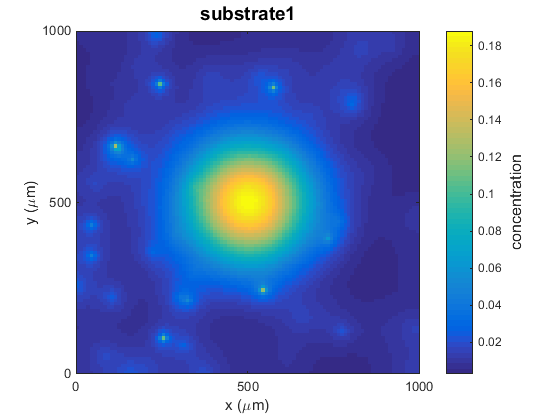
\includegraphics[width=0.3\textwidth]{./figures/sample_colormap.png} &
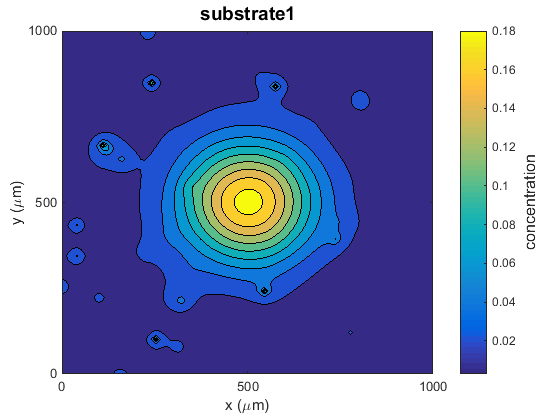
\includegraphics[width=0.3\textwidth]{./figures/sample_contour.png} &
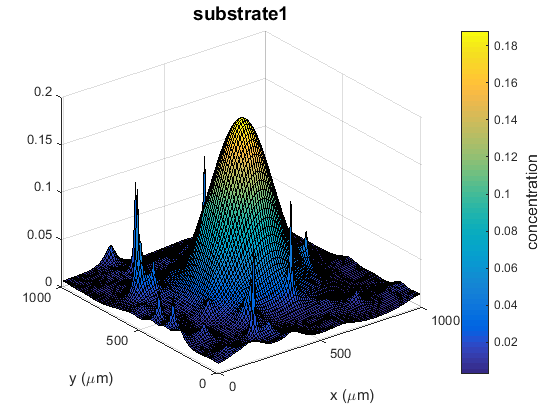
\includegraphics[width=0.3\textwidth]{./figures/sample_surface.png} \\
(a) & (b) & (c)\\
\end{tabular}
\caption{The visualization of middle cross section of the computational domain in Example 3 using provided Matlab scripts. (a) Colormap using \scriptsize{cross\_section\_colormap}, (b) contour using \scriptsize{cross\_section\_contour}, and (c) surface using \scriptsize{cross\_section\_surface}.  }
\label{Sample_matlab_figs}
\end{figure}


\section{Explicit solver}
\label{explicit_solver}
In addition to the implicit 3-D LOD solver, BioFVM also has an explicit solver for the cases that a user needs a much slower but more accurate solution. To use this solver, you need to register it with the microenvironment similar to the main solver:
\begin{verbatim}
microenvironment.diffusion_decay_solver = diffusion_decay_explicit_uniform_rates
\end{verbatim}

Note that the explicit solver needs a sufficiently small \verb:dt: to be stable.

\end{document} 